\section{Current product}
To give an overview of the progression of the project this section will provide an overview of what has been created during the sprint.
This overview will be split into two categories, to reflect the structure of the project: Networking and game.

\subsection{Networking}
The network aspect has been a big focus this sprint and has led to a better understanding of how the data should flow through the system (\autoref{sec:sprint2-deploymentdia}), and how the knowledge from sprint 1 about networking can be used to automatically find on-going games on the local network (\autoref{sec:accessonnetwork}).

From an implementation perspective, this sprint has introduced an initial version of the UDP host which is capable of transmitting Pozyx location data from the host computer to the game clients.
For the host, an initial console-based setup has been created, where the user can input the number of players, the location of the anchors as well as specify which tags are used in the game.
Additionally, the host can automatically re-order the list of entered anchors to ensure that they are sent to the clients in a clockwise manner, such that Unity can create a playing field mesh based on the coordinates.

\subsection{Game}
For the game aspect of the project, the most crucial parts have been implemented this sprint:\\
First of all, the game has been set up to support VR glasses by splitting the game view into two halves, one for each eye, as seen on \autoref{fig:initialvr}.

\begin{figure}[H]
	\centering
	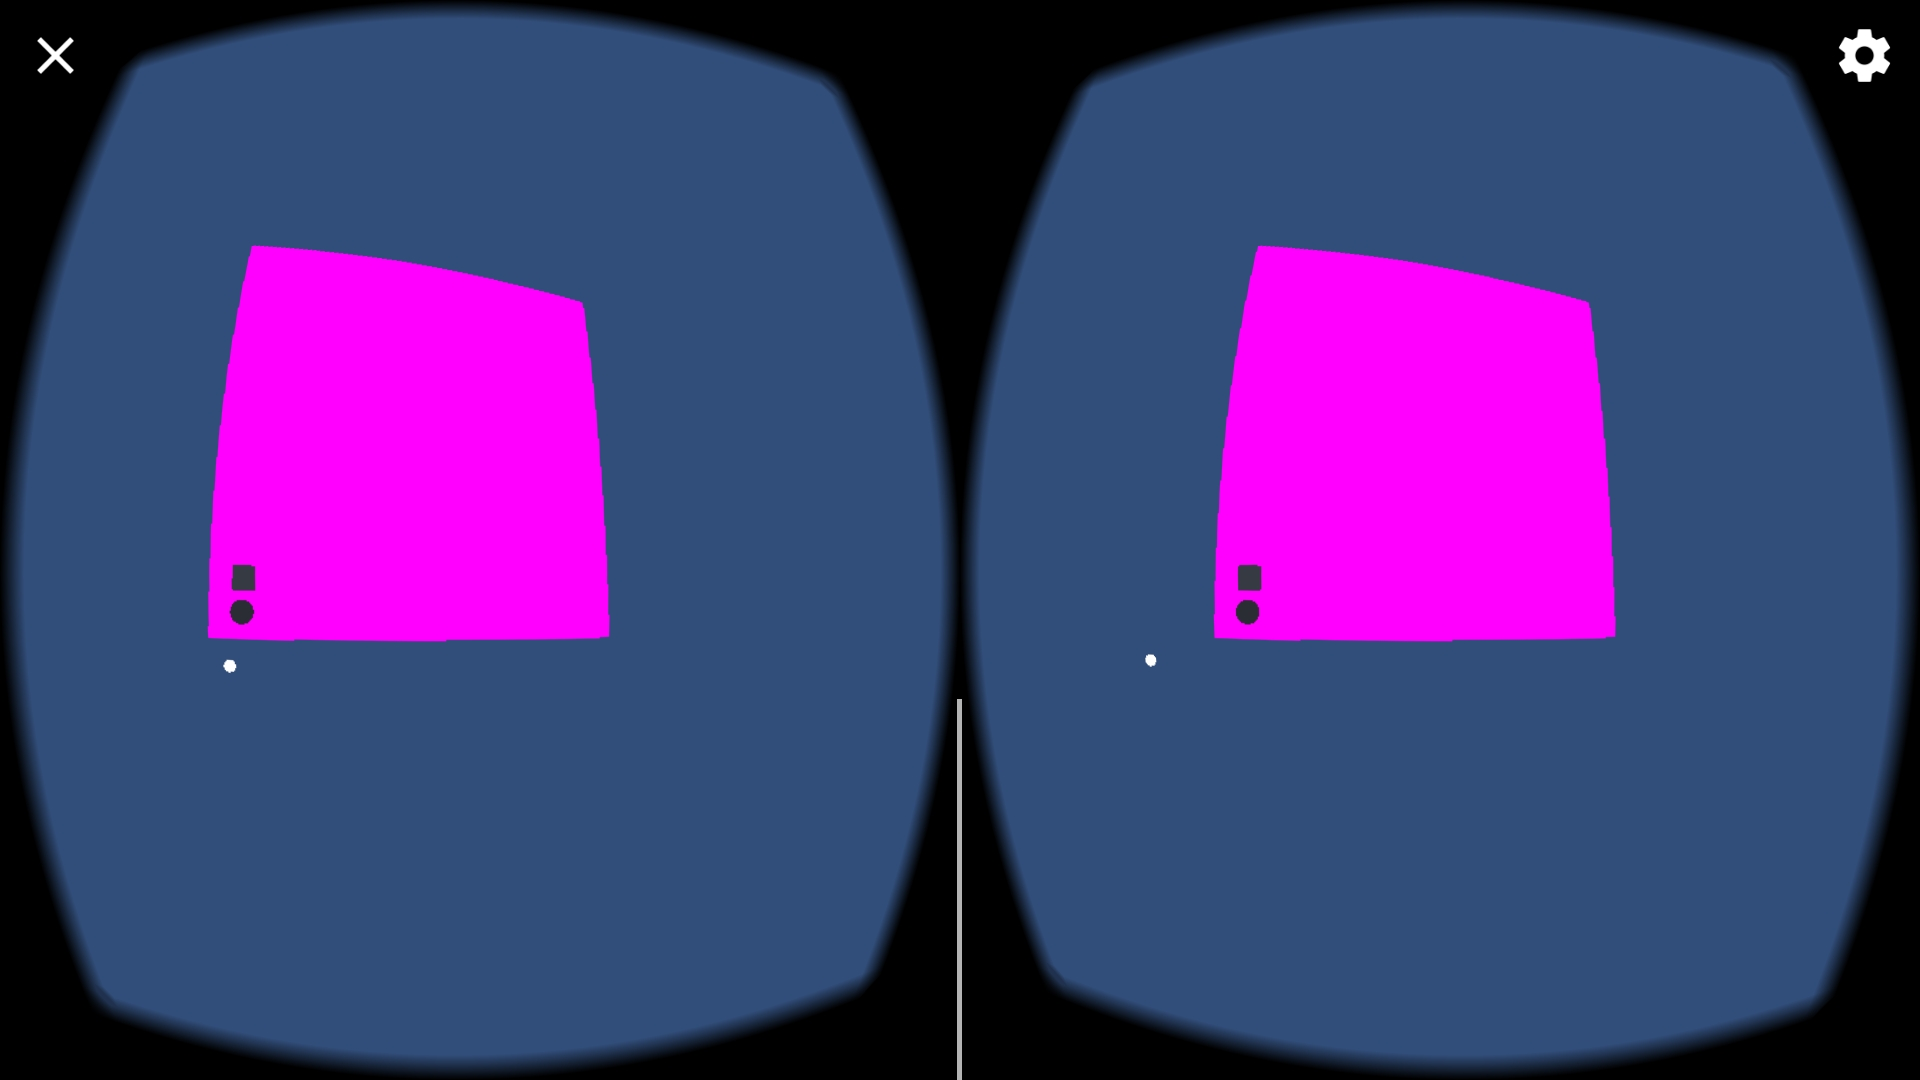
\includegraphics[width=0.6\linewidth]{sprint2/initialvr.jpg}
	\caption{The first implementation of VR}
	\label{fig:initialvr}
\end{figure}
\noindent
The game supports moving the players upon receiving new information from the host, but the connection between the two was not coupled together in this sprint.
Finally, an algorithm was implemented to generate the goal zones and ensure that they are placed fairly on the playing field.
